\chapter{Preliminaries}
\label{chapter:preliminaries}

In order to be able to explain the new \nonterm approach we have to declare, what \nonterm means, which programs are considered within this approach and present the construction of \gnas (GNAs), which builds the core of the approach. Furthermore we have to define a few structures we work on, we have to define what an \solver is and how it is used within this implementation.

%\section{Non-Termination}
%The definition of \nonterm is the most essential considering a technique proving it. Non-termination can be defined as a specific input to a program $p$, such that $p$ runs in an infinite loop.
%Proving termination is much harder than proving \nonterm, since we only have to determine one case, which fit's the condition of running into an infinite loop. \newline
%Non-termination is obviously still undecidable, since otherwise the halting problem would be decidable, nevertheless there are a large variety of possibilities to prove \nonterm as we will see in this paper.

\section{Integer Transition Systems}
\label{sec:its}
In order to apply the upcoming procedure we have to define what structure the approach works on. As described in \Cref{sec:aprove}, the C program is transferred into a symbolic execution graph. Afterwards, from each lasso of the graph an ITS is constructed. Here, a cycle is a lasso together with the path from the initial state to this cycle. Then, if we know that the resulting ITSs has the property that it is equivalent to the original program in its termination behaviour, we can prove non-termination of the original program by proving non-termination of one of the ITSs. Considering the following approach we will look at \itss of a special form shown in \Cref{fig:its-structure}.\newline
\begin{figure}[H]
	\begin{lstlisting}[escapechar=!]
		!$\overbrace{f_x}^{(1)} \qquad\qquad \rightarrow \overbrace{f_y}^{(2)} (v_1, \dots v_n) :|: cond_1$!
		!$\>f_y(\underbrace{v_1, \dots v_n}_{(3)}) \> \rightarrow \>\> f_y \>(\underbrace{v^\prime_1,\dots v^\prime_n}_{(3)})  :|: \underbrace{cond_2}_{(4)}$!
	\end{lstlisting}
	\caption{The structure of an \its considered in this thesis}
	\label{fig:its-structure}
\end{figure}

The \its shown in \Cref{fig:its-structure} consists of a set of structure elements, whose definition is necessary:
\begin{enumerate}[leftmargin=1]
	\item[(line 1)] The first line is the rewriting rule the program starts with and can be seen as a declaration of initial values of some variables. An example is shown in \Cref{fig:structure-example-TRS}.
	\item[(line 2)] A self-looping rule. Other looping rules will be presented in \Cref{sec:structure-improvement}.
	\item[(1)] The \textit{start function symbol} is the first symbol used, consisting of a function symbol without arguments. Further explanation in (line 1) and \Cref{fig:structure-example-TRS}.
	\item[(2)] A function symbol denoting a current program state
	\item[(3)] The arguments of a function symbol showing the update of the values by applying this rule. The value of $v^\prime_i$ is a linear update of the variables $v_j$, $1 \le j \le n$, in \stdLinInt. \footnote{The \stdLinInt has the following pattern: $ a_1*v_1 + \dots + a_n*v_n + c$, where $a_i , c \in \mathbb{Z}$, $1 \le i\le n$. }
%		Also it is important that $a_i * v_i$ has this order and not $v_i*a_i$} 
	\item[(4)] The conditional term of the form $\text{(in)equation}_1 \text{ \&\& } \dots \text{ \&\& } \text{(in)equation}_m$, $m \in \mathbb{N}$, where $\text{(in)equation}_i$ does not only contain the variables $v_j$, $1 \le j \le n$, but can also introduce new variables. The form of the (in)equalities is defined in \Cref{sec:derivation-guard}.	
\end{enumerate} 

A run of an ITS is the successive application of rules, starting from a start function symbol.
The termination of an \its is now defined as the absence of an infinite run, i.e. for every run we reach a state in which we can not apply any rule. Vice versa non-termination of an \its is defined as the existence of an infinite run.

%In general an \its can have rules of other forms, like $f_x(v_1, \dots v_n) \rightarrow f_y(v^\prime_1, \dots v^\prime_k) :|: cond$ where $n \ne k$ can occur, but these rules are for now not considered.

\section{Geometric Non-Termination Arguments}
Adapted from Jan Leikes and Matthias Heizmanns paper \textit{geometric non-termination arguments (GNA)} \cite{leike2014geometric} we will define the considered programs, define the division of these programs into \stem and \loopt and finally give the definition of \textit{geometric non-termination arguments}.

\subsection{Considered Programs}
The considered programs are not bound to a special programming language. The paper works on so called \textit{linear lasso programs}, which in fact are also used within \aprove. Instead of the linear lasso programs, \aprove represents them as ITSs, stated in \Cref{sec:aprove}. Because of the also stated conversion of the program into a \seg and because of the further analysis the applicability of GNAs is not bound to any programming language. \newline
In order to define the specific conditions under which we can use the approach, we choose the language \tool{Java} as an example.
\subsection{Structure}
\label{sec:structure}
The structure of the considered programs is quite simple. It contains an optional initialization  of the used variables and a \code{while}-loop. Even though \tool{C} would not accept the usage of a variable without declaration, the conversion to \llvm would still be sound. An example of a linear lasso program in \tool{C} is shown in \Cref{fig:structure-example-java}. 
\begin{itemize}
	\item The \stem: \newline
		The declaration and optional initialization of variables used within the \code{while}-loop. In \Cref{fig:structure-example-java} lines 3 and 4 are considered the \stem. Only $b$ is initialized with a value.
	\item The guard: \newline
		The guard of the \code{while}-loop is essential to restrict the variable $a$ as we will see in \Cref{sec:stem-var}. With the restriction of $a+b\ge 4 $ we can prove termination for an initial value of $a < 3$ without further analysis, and also, in order to prove \nonterm, assume that initially $a \ge 3$.
	\item The linear updates: \newline
		The updates of the variables within the \code{while}-loop are the most essential part for termination, since their values determine if the guard still holds. The approach only works with linear updates of the variables, so for every variable $v_i$ where $1\le i\le n$ we can have an update of the form $v_i=a_1*v_1+...+a_n*v_n+c$ with $a_i \in \mathbb{Z}$ for $1 \le i \le n$ and $c \in \mathbb{Z}$.
\end{itemize} 

\begin{figure}[h]
	\begin{lstlisting}[language = java, escapechar = !, linewidth=0.6\linewidth]
	int main(){
		
		int a;!\tikz[remember picture] \node [] (a) {};!
		int b=1;!\tikz[remember picture] \node [] (b) {};!
		
		while(a+b>=4){! \tikz[remember picture] \node [] (c) {}; !
			a=3*a+b;!\tikz[remember picture] \node [] (d) {}; !
			b=2*b-5;!\tikz[remember picture] \node [] (e) {}; !
		}
	}		
	\end{lstlisting}
	\begin{tikzpicture}[remember picture, overlay, 
		every edge/.append style = {dashedarrow},
		every node/.append style = {explNode},
	text width = 2.5cm ]
		\node[above right = .2cm and 3.1 cm of a] (A) {the \textit{STEM}};
		\draw[rounded corners=5pt] (A.west) edge (a.east);
		\draw (A.west) edge (b.east);
		
		\node[below = of A, right = of c] (B) {the guard};
		\draw (B.west) edge (c.east);
		
		\node[right = 4cm of d, below = of B] (C) {the linear update};
		\draw (C.west) edge (d.east);
		\draw (C.west) edge (e.east);
	\end{tikzpicture}
	\caption{A linear lasso program fulfilling the conditions mentioned in \Cref{sec:structure} to be applicable}
	\label{fig:structure-example-java}
\end{figure}
The guard and linear updates together form the so called \loopt. 

%Through the in \Cref{sec:its} described procedure and given structure we receive the to \Cref{fig:structure-example-java} corresponding \its shown in \Cref{fig:structure-example-TRS}. 
The program from \Cref{fig:structure-example-java} can be transformed into the ITS shown in \Cref{fig:structure-example-TRS}, which is conform to the structure described in \Cref{sec:structure}.
As we can see, the original program can be recognized quite easily. The first rule in line 1 represents the \stem, while the second line forms the \loopt. \newline

%TODO: richtig formatieren
\begin{figure}[H]	
	\begin{lstlisting}[linewidth=1.1\textwidth, escapechar = !]
!$\overbrace{f_1	     \rightarrow f_2(1+3*v_1,-3)   :|: v_1>2 \text{ \&\& } 8<3*v_1}^{\text{\stem}}$!
!$f_2(v_1,v_2) \rightarrow f_2(3*v_1+v_2,v_3) :|: v_1 + v_2 > 3 \text{ \&\& } v_1 > 6 \text{ \&\& } 3 * v_1 > 20 \text{ \&\& }$!
!$\underbrace{\text{\qquad\qquad\qquad\qquad\qquad\qquad}}_{\text{linear update}}$!		!$\underbrace{ 5 + v_3 = 2 * v_2 \text{ \&\& } v_3 < -10\text{\qquad\qquad\qquad} }_{\text{guards}}$!
!$\underbrace{\text{\qquad\qquad\qquad\qquad\qquad\qquad\qquad\qquad\qquad\qquad\qquad\qquad\qquad\qquad\qquad\qquad}}_{\text{\loopt}}$!
	\end{lstlisting}

	\caption{The \its corresponding to the \tool{Java} program in \Cref{fig:structure-example-java}}
	\label{fig:structure-example-TRS}
\end{figure}

Neglecting the conditional terms for now, we initialize  $v^\prime_2$, which is the second argument of $f_2$, in line 1 to the value of -3, 
because during the construction of the \seg, \aprove always unrolls the first iteration of the \loopt. Therefore, the \stem computed by \aprove will always contain the first execution of the \loopt. Starting with $b=1$ one step would be the computation of $b = 2*1-5=-3$. The definition of $v^\prime_1$ is more difficult and will be shown within \Cref{sec:stem}.
%TODO: b von 1 zu -3
Also the update of  $v^\prime_1$, which is the first argument of $f_2$, within line 2 is the same as in \Cref{fig:structure-example-java} line 7. The definition of the second argument of $f_2$, $v^\prime_2 = v_3$, is fundamental and not as simple as $v^\prime_1$, since $v_3$ is a new variable introduced within the guards through the equality $5+v_3=2*v_2$. The handling of such variables will be explained in \Cref{sec:derivation-guard} and \Cref{sec:derivation-update}. \newline

\subsection{Preliminary Definitions}
In order to be able to define the key element of this approach, the \gna, we have to define a number of matrices and constant vectors, which are used to derive such a \gna. 

\begin{definition}[\stem]
	The \stem is denoted as a vector $x \in \mathbb{Z}^n$, where $n$ is the arity of the function symbol at the right hand side of the rule representing the \stem of the \its. The values of $x$ can be constants or restricted by a (possibly empty) conjunction of conditions. 
\end{definition}
Examples of the \stem are shown within \Cref{sec:stem}.

\begin{definition}[Guard Matrix, Guard Constants]
	\label{def:guard}
	Let $n \in \mathbb{N}$ be the number of distinct variables of the \loopt rules left hand side, $v_j$, $1 \le j \le n$, the $j$-th distinct variable occurring on the left hand side of the rule, $m \in \mathbb{N}$ be the number of guards not containing equality, $r_i$, $1\le i \le m$, the $i$-th guard, $a_{i,j} \in \mathbb{Z}$, $1 \le i \le m$ and $1\le j \le n$, the coefficient of $v_j$ in $r_i$ and $c_i \in \mathbb{Z}$ be the constant term within $r_i$.
	
	Then the \guardmatrix $G \in \mathbb{Z}^{m\times n}$ is defined as $G_{i,j}=a_{i,j} $ and \guardconstants $g \in \mathbb{Z}^m$ are defined as $g_i = c_i$.
	
	Newly introduced variables must not be represented by a column of the \guardmatrix, but create substitutions further discussed in \Cref{sec:stem-var}, \Cref{sec:derivation-guard} and \Cref{sec:derivation-update}.
\end{definition}

\begin{example}
	\label{ex:guardmatrix-and-constants}
	First we normalize every guard $r_i$ to the form $a_{i,1}v_1+\dots a_{i,n}v_n \le c$. For example the guard $r_1$ in the following way:
	\begin{center}
		$r_1 \Leftrightarrow v_1+v_2 > 3  \Leftrightarrow -v_1-v_2 < -3 \Leftrightarrow -v_1-v_2 \le -4$
	\end{center}
	The necessity and computation of the normalization is explained within \Cref{sec:derivation-guard}.\newline
	Since the coefficient of $v_1$ is $-1$ and of $v_2$ is also $-1$ we can set the entries $G_{1,1} = G_{1,2}=-1$.
	Iterating over all $r_i$ we derive the corresponding \guardmatrix to \Cref{fig:structure-example-TRS} is $G = \begin{pmatrix} -1 & -1 \\ -1 & 0 \\ -3 & 0 \\ 0 & 2 \end{pmatrix}$.
	The constant factor of a guard $r_i$ is the right hand side of the inequation. So the constant of $r_1=-4$. Iterating over all $r_i$ we derive the \guardconstants are $g= \begin{pmatrix} -4 \\ -7 \\ -21 \\ -6 \end{pmatrix}$.	
\end{example}

\begin{definition}[Update Matrix, Update Constants]
	\label{def:update}
	Let $n \in \mathbb{N}$ be the number of distinct variables of the \loopt rules left hand side, $v_j$, $1 \le j \le n$, the $j$-th distinct	variables of the \loopt rules left hand side, $m \in \mathbb{N}$ the arity of the function symbol of the right hand side, $v^\prime_i$, $1 \le i \le m$, the $i$-th argument of the right hand side function, $a_{i,j} \in \mathbb{Z}$, $1 \le i \le m$ and $1 \le j \le n$, be the coefficient of variable $v_j$ in $v^\prime_i$ and $c_i \in \mathbb{Z}$, $1 \le i \le m$, the constant term of $v^\prime_i$. \newline
	Then the \updatematrix $U \in \mathbb{Z}^{m \times n}$ is defined as $U_{i,j}=a_{i,j}$ and the \updateconstants $u \in \mathbb{Z}^m$ are defined as $u_i = c_i$.
\end{definition}
Regarding the new variable $v_3$, we have to substitute in order to keep the desired size of the matrix. This procedure is further defined within \Cref{sec:derivation-guard} and \Cref{sec:derivation-update}.

\begin{example}
	\label{ex:updatematrix-and-constants}
	Referring to the \its from \Cref{fig:structure-example-TRS} we have to substitute $v_3$.
	\begin{center}
		$5+v_3=2*v_2 \Leftrightarrow v_3=2*v_2-5$
	\end{center}
	So we substitute $v_3$ in the second argument and receive the arguments $2*v_1+v_2$ and $2*v_2-5$.
	The corresponding \updatematrix is therefore $U = \begin{pmatrix} 3 & 1 \\ 0 & 2 \end{pmatrix}$ and the \updateconstants are $u = \begin{pmatrix} 0 \\ -5 \end{pmatrix}$.
	
	The detailed derivation of substitutions is explained in \Cref{sec:derivation-update}.
\end{example}

\begin{definition}[Iteration Matrix, Iteration Constants]
	\label{def:iteration}
	Let $G$ be the \guardmatrix, $g$ the \guardconstants, $U$ the \updatematrix, $u$ the \updateconstants, $n\in \mathbb{N}$ the number of variables and $m \in \mathbb{N}$ the number of conditional terms. \newline
	Furthermore let \textbf{0} be a matrix of the size of $G$ with only zero entries and $I$ denote the identity matrix having the same dimension as $U$. \newline
	The \iterationmatrix $A \in \mathbb{Z}^{2n+m \times 2n}$, which computes one complete execution of the \loopt, and the \iterationconstants $b\in \mathbb{Z}^{2n+m} $ are defined as
	\begin{figure}[H]
		\centering
		$A = \begin{pmatrix} G & \textbf{0} \\ U & -I \\ -U & I \end{pmatrix}$ and $b = \begin{pmatrix} g \\ -u \\ u \end{pmatrix}$ \cite{leike2014geometric}
	\end{figure}	
\end{definition}

\begin{example}
	Taking the \guardmatrix $G$ and \guardconstants $g$ from \Cref{ex:guardmatrix-and-constants}, and the \guardmatrix $U$ and \updateconstants $u$ from \Cref{ex:updatematrix-and-constants} and computing the \iterationmatrix $A$ and \iterationconstants $b$ by inserting the matrices and vectors into the formula of \Cref{def:iteration} we get: \newline
	\begin{center}
		$A = \begin{pmatrix} G & \textbf{0} \\ U & -I \\ -U & I \end{pmatrix} \Rightarrow 
		\begin{pmatrix} 
			-1 & -1 & 0 & 0 \\
			-1 & 0 & 0 & 0 \\
			-3 & 0 & 0 & 0\\
			0 & 2 & 0 & 0 \\
			3 & 1 & -1 & 0 \\
			0 & 2 & 0 & -1 \\
			-3 & -1 & 1 & 0 \\
			0 & -2 & 0 & 1 \\
		\end{pmatrix}$ and 
		$b = \begin{pmatrix} g \\ -u \\ u \end{pmatrix} \Rightarrow \begin{pmatrix}
			-4 \\ -7 \\-21\\-6\\ 0 \\ 5 \\ 0 \\ -5
		\end{pmatrix}$
	\end{center}
\end{example}

\begin{definition}[LOOP]
	The \loopt is defined as a tuple $(A, b)$, where $A$ is the \iterationmatrix and $b$ the \iterationconstants of an \its.
\end{definition}

Now we can define the key element, which was originally defined for linear lasso programs. 

\begin{definition}[Geometric Non-Termination Argument]
	\label{def:gna}
	A tuple of the form:
	\begin{figure}[H]
		\centering
		$(x, y_1, \dots, y_k, \lambda_1, \dots, \lambda_k, \mu_1, \dots, \mu_{k-1})$
	\end{figure}  
	\vspace{-1em}
	is called a \gna (GNA) of size $k$ for a program $(\stem, \loopt)$ with $n$ variables iff all of the following statements hold:
	\begin{itemize}
		\setlength{\itemindent}{1in}
		\item[(domain)] $x, y_1, \dots, y_k \in \mathbb{R}^n$, $\lambda_1, \dots \lambda_k, \mu_1, \dots \mu_{k-1} \ge 0$
		\item[(init)] x represents a valid \stem
		\item[(point)] $A\begin{pmatrix} x \\ x + \sum_i y_i \end{pmatrix} \le b$
		\item[(ray)] $A\begin{pmatrix} y_i \\ \lambda_i y_i + \mu_{i-1} y_{i-1} \end{pmatrix} \le 0$ for all $1 \le i \le k$
	\end{itemize}
	Here $y_0 = \mu_0 = 0$ is set for the ray instead of a case distinction for $i=1$ \cite{leike2014geometric}.
\end{definition}
The validity of the \initc refers to the possibility of different valid STEMs, further defined in \Cref{sec:stem-var}.
An intuitive interpretation of the \pointc is the validity of entering the corresponding loop. If the \pointc does not hold the \its is unable to enter the loop and therefore we can not argue about a \nonterm loop. One iteration of the \rayc is computed based on the previous iteration through the $y_{i-1}$. Also the stated initialization of $y_0=0$ is very intuitive since $i=1$ represents the first iteration and therefore no previous iteration exists. The similarity to the geometric series used within \cite{leike2014geometric} is quite obvious. The whole \rayc can therefore intuitively interpreted as the computation, which keeps the program within this loop. 
%TODO: die größe...
%The size of the GNA defines the steps of computation since we reach and 
\begin{example}
	A valid GNA to the computed matrices of \Cref{ex:guardmatrix-and-constants} and \Cref{ex:updatematrix-and-constants} is:\newline
	\begin{figure}[H]
		\centering
		\begin{tabular}{|c|c|c|c|c|c|}
			\hline
			\stem & $y_1$ & $y_2$ & $\lambda_1$ & $\lambda_2$ & $\mu_1$ \\ \hline
			$\begin{pmatrix} 10 \\ -3 \end{pmatrix}$ & $\begin{pmatrix} 9 \\ 0 \end{pmatrix}$ & $\begin{pmatrix} 8 \\ -8 \end{pmatrix}$ & 3 & 2 & 0 \\ \hline
		\end{tabular}
	\end{figure}
\end{example}
The proof of the example being valid is written in \Cref{sec:verification-of-gna}.
The usage of such a \gna is justified by the following sentence:
\begin{satz}
	\label{sen:gna-nonterm}
	If a \gna for a program $p$ exists, then $p$ does not terminate \cite{leike2014geometric}.
\end{satz}

\section{Reverse-Polish-Notation-Tree}
\label{sec:rpntree}
Within the procedure of deriving a \gna it happens that we get a mathematical term in the so-called \textit{Polish Notation} or \textit{Reverse Polish Notation in prefix notation}, which is a special form of rewriting a, in our case linear, expression to compute the solution efficiently using a stack \cite{wikirpn}. We use this kind of notation to parse it into our own tree structure to do further analysis.

As shown in \Cref{dia:RPN-classdiagram} we have an \code{abstract} root, subclasses for every occurring type of element within the \its, a \code{static} parsing of a given term and an exception for parsing exceptions.
An example of the \rpntree's usage is shown in \Cref{ex:rpntree}

\begin{figure}[H]
	\centering
	% Graphic for TeX using PGF
% Title: D:\Dokumente\GitHub\Bachelorarbeit\Arbeitstagebuch\src\04.07.2017-RPNTree-classdiagram.dia
% Creator: Dia v0.97.2
% CreationDate: Wed Aug 30 19:22:10 2017
% For: Timo Bergerbusch
% \usepackage{tikz}
% The following commands are not supported in PSTricks at present
% We define them conditionally, so when they are implemented,
% this pgf file will use them.
\ifx\du\undefined
  \newlength{\du}
\fi
\setlength{\du}{15\unitlength}
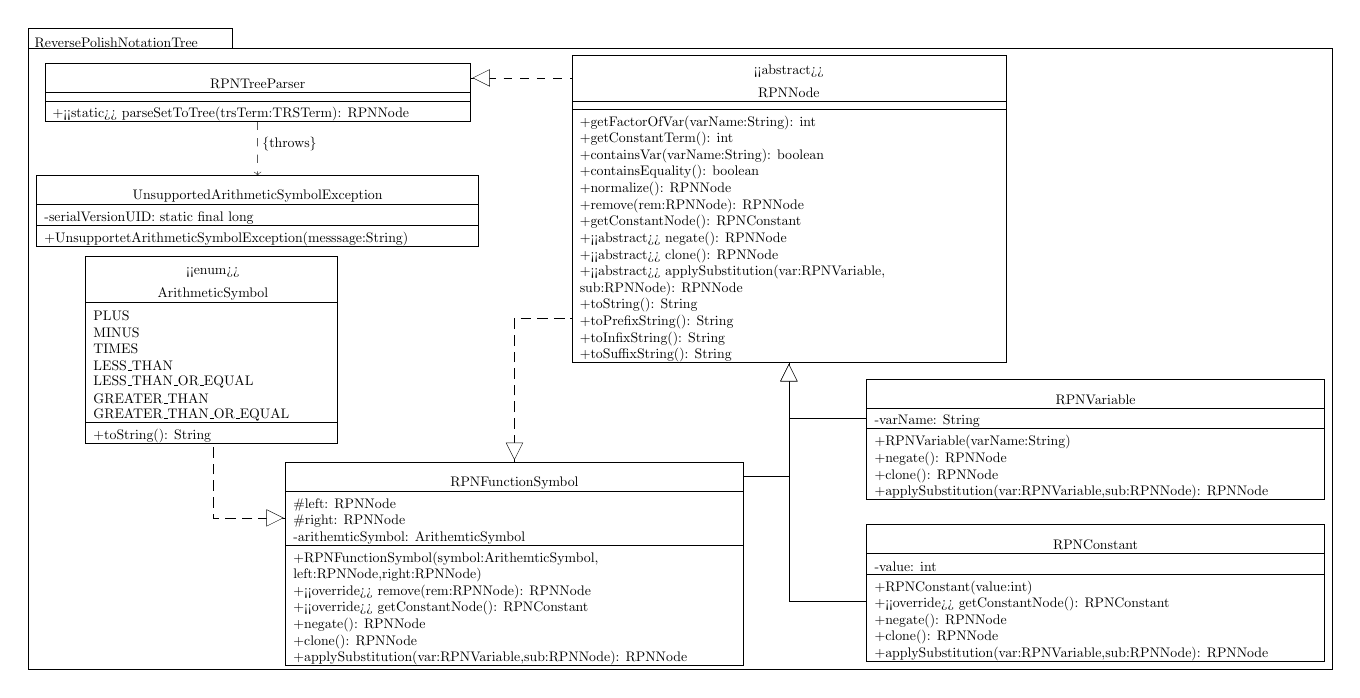
\begin{tikzpicture}[scale=0.5, every node/.style={scale=0.5}]
\pgftransformxscale{1.000000}
\pgftransformyscale{-1.000000}
\definecolor{dialinecolor}{rgb}{0.000000, 0.000000, 0.000000}
\pgfsetstrokecolor{dialinecolor}
\definecolor{dialinecolor}{rgb}{1.000000, 1.000000, 1.000000}
\pgfsetfillcolor{dialinecolor}
\pgfsetlinewidth{0.010000\du}
\pgfsetdash{}{0pt}
\definecolor{dialinecolor}{rgb}{1.000000, 1.000000, 1.000000}
\pgfsetfillcolor{dialinecolor}
\fill (-2.412990\du,34.090900\du)--(-2.412990\du,64.000000\du)--(60.422652\du,64.000000\du)--(60.422652\du,34.090900\du)--cycle;
\definecolor{dialinecolor}{rgb}{0.000000, 0.000000, 0.000000}
\pgfsetstrokecolor{dialinecolor}
\draw (-2.412990\du,34.090900\du)--(-2.412990\du,64.000000\du)--(60.422652\du,64.000000\du)--(60.422652\du,34.090900\du)--cycle;
\definecolor{dialinecolor}{rgb}{1.000000, 1.000000, 1.000000}
\pgfsetfillcolor{dialinecolor}
\fill (-2.412990\du,33.090900\du)--(-2.412990\du,34.090900\du)--(7.412010\du,34.090900\du)--(7.412010\du,33.090900\du)--cycle;
\definecolor{dialinecolor}{rgb}{0.000000, 0.000000, 0.000000}
\pgfsetstrokecolor{dialinecolor}
\draw (-2.412990\du,33.090900\du)--(-2.412990\du,34.090900\du)--(7.412010\du,34.090900\du)--(7.412010\du,33.090900\du)--cycle;
% setfont left to latex
\definecolor{dialinecolor}{rgb}{0.000000, 0.000000, 0.000000}
\pgfsetstrokecolor{dialinecolor}
\node[anchor=west] at (-2.312990\du,33.790900\du){ReversePolishNotationTree};
\pgfsetlinewidth{0.010000\du}
\pgfsetdash{}{0pt}
\definecolor{dialinecolor}{rgb}{1.000000, 1.000000, 1.000000}
\pgfsetfillcolor{dialinecolor}
\fill (23.800000\du,34.400000\du)--(23.800000\du,36.600000\du)--(44.705000\du,36.600000\du)--(44.705000\du,34.400000\du)--cycle;
\definecolor{dialinecolor}{rgb}{0.000000, 0.000000, 0.000000}
\pgfsetstrokecolor{dialinecolor}
\draw (23.800000\du,34.400000\du)--(23.800000\du,36.600000\du)--(44.705000\du,36.600000\du)--(44.705000\du,34.400000\du)--cycle;
% setfont left to latex
\definecolor{dialinecolor}{rgb}{0.000000, 0.000000, 0.000000}
\pgfsetstrokecolor{dialinecolor}
\node at (34.252500\du,35.160000\du){<<abstract>>};
% setfont left to latex
\definecolor{dialinecolor}{rgb}{0.000000, 0.000000, 0.000000}
\pgfsetstrokecolor{dialinecolor}
\node at (34.252500\du,36.200000\du){RPNNode};
\definecolor{dialinecolor}{rgb}{1.000000, 1.000000, 1.000000}
\pgfsetfillcolor{dialinecolor}
\fill (23.800000\du,36.600000\du)--(23.800000\du,37.000000\du)--(44.705000\du,37.000000\du)--(44.705000\du,36.600000\du)--cycle;
\definecolor{dialinecolor}{rgb}{0.000000, 0.000000, 0.000000}
\pgfsetstrokecolor{dialinecolor}
\draw (23.800000\du,36.600000\du)--(23.800000\du,37.000000\du)--(44.705000\du,37.000000\du)--(44.705000\du,36.600000\du)--cycle;
\definecolor{dialinecolor}{rgb}{1.000000, 1.000000, 1.000000}
\pgfsetfillcolor{dialinecolor}
\fill (23.800000\du,37.000000\du)--(23.800000\du,49.200000\du)--(44.705000\du,49.200000\du)--(44.705000\du,37.000000\du)--cycle;
\definecolor{dialinecolor}{rgb}{0.000000, 0.000000, 0.000000}
\pgfsetstrokecolor{dialinecolor}
\draw (23.800000\du,37.000000\du)--(23.800000\du,49.200000\du)--(44.705000\du,49.200000\du)--(44.705000\du,37.000000\du)--cycle;
% setfont left to latex
\definecolor{dialinecolor}{rgb}{0.000000, 0.000000, 0.000000}
\pgfsetstrokecolor{dialinecolor}
\node[anchor=west] at (23.950000\du,37.660000\du){+getFactorOfVar(varName:String): int};
% setfont left to latex
\definecolor{dialinecolor}{rgb}{0.000000, 0.000000, 0.000000}
\pgfsetstrokecolor{dialinecolor}
\node[anchor=west] at (23.950000\du,38.460000\du){+getConstantTerm(): int};
% setfont left to latex
\definecolor{dialinecolor}{rgb}{0.000000, 0.000000, 0.000000}
\pgfsetstrokecolor{dialinecolor}
\node[anchor=west] at (23.950000\du,39.260000\du){+containsVar(varName:String): boolean};
% setfont left to latex
\definecolor{dialinecolor}{rgb}{0.000000, 0.000000, 0.000000}
\pgfsetstrokecolor{dialinecolor}
\node[anchor=west] at (23.950000\du,40.060000\du){+containsEquality(): boolean};
% setfont left to latex
\definecolor{dialinecolor}{rgb}{0.000000, 0.000000, 0.000000}
\pgfsetstrokecolor{dialinecolor}
\node[anchor=west] at (23.950000\du,40.860000\du){+normalize(): RPNNode};
% setfont left to latex
\definecolor{dialinecolor}{rgb}{0.000000, 0.000000, 0.000000}
\pgfsetstrokecolor{dialinecolor}
\node[anchor=west] at (23.950000\du,41.660000\du){+remove(rem:RPNNode): RPNNode};
% setfont left to latex
\definecolor{dialinecolor}{rgb}{0.000000, 0.000000, 0.000000}
\pgfsetstrokecolor{dialinecolor}
\node[anchor=west] at (23.950000\du,42.460000\du){+getConstantNode(): RPNConstant};
% setfont left to latex
\definecolor{dialinecolor}{rgb}{0.000000, 0.000000, 0.000000}
\pgfsetstrokecolor{dialinecolor}
\node[anchor=west] at (23.950000\du,43.260000\du){+<<abstract>> negate(): RPNNode};
% setfont left to latex
\definecolor{dialinecolor}{rgb}{0.000000, 0.000000, 0.000000}
\pgfsetstrokecolor{dialinecolor}
\node[anchor=west] at (23.950000\du,44.060000\du){+<<abstract>> clone(): RPNNode};
% setfont left to latex
\definecolor{dialinecolor}{rgb}{0.000000, 0.000000, 0.000000}
\pgfsetstrokecolor{dialinecolor}
\node[anchor=west] at (23.950000\du,44.860000\du){+<<abstract>> applySubstitution(var:RPNVariable,};
\definecolor{dialinecolor}{rgb}{0.000000, 0.000000, 0.000000}
\pgfsetstrokecolor{dialinecolor}
\node[anchor=west] at (23.950000\du,45.660000\du){                                sub:RPNNode): RPNNode};
% setfont left to latex
\definecolor{dialinecolor}{rgb}{0.000000, 0.000000, 0.000000}
\pgfsetstrokecolor{dialinecolor}
\node[anchor=west] at (23.950000\du,46.460000\du){+toString(): String};
% setfont left to latex
\definecolor{dialinecolor}{rgb}{0.000000, 0.000000, 0.000000}
\pgfsetstrokecolor{dialinecolor}
\node[anchor=west] at (23.950000\du,47.260000\du){+toPrefixString(): String};
% setfont left to latex
\definecolor{dialinecolor}{rgb}{0.000000, 0.000000, 0.000000}
\pgfsetstrokecolor{dialinecolor}
\node[anchor=west] at (23.950000\du,48.060000\du){+toInfixString(): String};
% setfont left to latex
\definecolor{dialinecolor}{rgb}{0.000000, 0.000000, 0.000000}
\pgfsetstrokecolor{dialinecolor}
\node[anchor=west] at (23.950000\du,48.860000\du){+toSuffixString(): String};
\pgfsetlinewidth{0.010000\du}
\pgfsetdash{}{0pt}
\definecolor{dialinecolor}{rgb}{1.000000, 1.000000, 1.000000}
\pgfsetfillcolor{dialinecolor}
\fill (38.000000\du,50.000000\du)--(38.000000\du,51.400000\du)--(60.060000\du,51.400000\du)--(60.060000\du,50.000000\du)--cycle;
\definecolor{dialinecolor}{rgb}{0.000000, 0.000000, 0.000000}
\pgfsetstrokecolor{dialinecolor}
\draw (38.000000\du,50.000000\du)--(38.000000\du,51.400000\du)--(60.060000\du,51.400000\du)--(60.060000\du,50.000000\du)--cycle;
% setfont left to latex
\definecolor{dialinecolor}{rgb}{0.000000, 0.000000, 0.000000}
\pgfsetstrokecolor{dialinecolor}
\node at (49.030000\du,51.000000\du){RPNVariable};
\definecolor{dialinecolor}{rgb}{1.000000, 1.000000, 1.000000}
\pgfsetfillcolor{dialinecolor}
\fill (38.000000\du,51.400000\du)--(38.000000\du,52.400000\du)--(60.060000\du,52.400000\du)--(60.060000\du,51.400000\du)--cycle;
\definecolor{dialinecolor}{rgb}{0.000000, 0.000000, 0.000000}
\pgfsetstrokecolor{dialinecolor}
\draw (38.000000\du,51.400000\du)--(38.000000\du,52.400000\du)--(60.060000\du,52.400000\du)--(60.060000\du,51.400000\du)--cycle;
% setfont left to latex
\definecolor{dialinecolor}{rgb}{0.000000, 0.000000, 0.000000}
\pgfsetstrokecolor{dialinecolor}
\node[anchor=west] at (38.150000\du,52.060000\du){-varName: String};
\definecolor{dialinecolor}{rgb}{1.000000, 1.000000, 1.000000}
\pgfsetfillcolor{dialinecolor}
\fill (38.000000\du,52.400000\du)--(38.000000\du,55.800000\du)--(60.060000\du,55.800000\du)--(60.060000\du,52.400000\du)--cycle;
\definecolor{dialinecolor}{rgb}{0.000000, 0.000000, 0.000000}
\pgfsetstrokecolor{dialinecolor}
\draw (38.000000\du,52.400000\du)--(38.000000\du,55.800000\du)--(60.060000\du,55.800000\du)--(60.060000\du,52.400000\du)--cycle;
% setfont left to latex
\definecolor{dialinecolor}{rgb}{0.000000, 0.000000, 0.000000}
\pgfsetstrokecolor{dialinecolor}
\node[anchor=west] at (38.150000\du,53.060000\du){+RPNVariable(varName:String)};
% setfont left to latex
\definecolor{dialinecolor}{rgb}{0.000000, 0.000000, 0.000000}
\pgfsetstrokecolor{dialinecolor}
\node[anchor=west] at (38.150000\du,53.860000\du){+negate(): RPNNode};
% setfont left to latex
\definecolor{dialinecolor}{rgb}{0.000000, 0.000000, 0.000000}
\pgfsetstrokecolor{dialinecolor}
\node[anchor=west] at (38.150000\du,54.660000\du){+clone(): RPNNode};
% setfont left to latex
\definecolor{dialinecolor}{rgb}{0.000000, 0.000000, 0.000000}
\pgfsetstrokecolor{dialinecolor}
\node[anchor=west] at (38.150000\du,55.460000\du){+applySubstitution(var:RPNVariable,sub:RPNNode): RPNNode};
\pgfsetlinewidth{0.010000\du}
\pgfsetdash{}{0pt}
\definecolor{dialinecolor}{rgb}{1.000000, 1.000000, 1.000000}
\pgfsetfillcolor{dialinecolor}
\fill (38.000000\du,57.000000\du)--(38.000000\du,58.400000\du)--(60.060000\du,58.400000\du)--(60.060000\du,57.000000\du)--cycle;
\definecolor{dialinecolor}{rgb}{0.000000, 0.000000, 0.000000}
\pgfsetstrokecolor{dialinecolor}
\draw (38.000000\du,57.000000\du)--(38.000000\du,58.400000\du)--(60.060000\du,58.400000\du)--(60.060000\du,57.000000\du)--cycle;
% setfont left to latex
\definecolor{dialinecolor}{rgb}{0.000000, 0.000000, 0.000000}
\pgfsetstrokecolor{dialinecolor}
\node at (49.030000\du,58.000000\du){RPNConstant};
\definecolor{dialinecolor}{rgb}{1.000000, 1.000000, 1.000000}
\pgfsetfillcolor{dialinecolor}
\fill (38.000000\du,58.400000\du)--(38.000000\du,59.400000\du)--(60.060000\du,59.400000\du)--(60.060000\du,58.400000\du)--cycle;
\definecolor{dialinecolor}{rgb}{0.000000, 0.000000, 0.000000}
\pgfsetstrokecolor{dialinecolor}
\draw (38.000000\du,58.400000\du)--(38.000000\du,59.400000\du)--(60.060000\du,59.400000\du)--(60.060000\du,58.400000\du)--cycle;
% setfont left to latex
\definecolor{dialinecolor}{rgb}{0.000000, 0.000000, 0.000000}
\pgfsetstrokecolor{dialinecolor}
\node[anchor=west] at (38.150000\du,59.060000\du){-value: int};
\definecolor{dialinecolor}{rgb}{1.000000, 1.000000, 1.000000}
\pgfsetfillcolor{dialinecolor}
\fill (38.000000\du,59.400000\du)--(38.000000\du,63.600000\du)--(60.060000\du,63.600000\du)--(60.060000\du,59.400000\du)--cycle;
\definecolor{dialinecolor}{rgb}{0.000000, 0.000000, 0.000000}
\pgfsetstrokecolor{dialinecolor}
\draw (38.000000\du,59.400000\du)--(38.000000\du,63.600000\du)--(60.060000\du,63.600000\du)--(60.060000\du,59.400000\du)--cycle;
% setfont left to latex
\definecolor{dialinecolor}{rgb}{0.000000, 0.000000, 0.000000}
\pgfsetstrokecolor{dialinecolor}
\node[anchor=west] at (38.150000\du,60.060000\du){+RPNConstant(value:int)};
% setfont left to latex
\definecolor{dialinecolor}{rgb}{0.000000, 0.000000, 0.000000}
\pgfsetstrokecolor{dialinecolor}
\node[anchor=west] at (38.150000\du,60.860000\du){+<<override>> getConstantNode(): RPNConstant};
% setfont left to latex
\definecolor{dialinecolor}{rgb}{0.000000, 0.000000, 0.000000}
\pgfsetstrokecolor{dialinecolor}
\node[anchor=west] at (38.150000\du,61.660000\du){+negate(): RPNNode};
% setfont left to latex
\definecolor{dialinecolor}{rgb}{0.000000, 0.000000, 0.000000}
\pgfsetstrokecolor{dialinecolor}
\node[anchor=west] at (38.150000\du,62.460000\du){+clone(): RPNNode};
% setfont left to latex
\definecolor{dialinecolor}{rgb}{0.000000, 0.000000, 0.000000}
\pgfsetstrokecolor{dialinecolor}
\node[anchor=west] at (38.150000\du,63.260000\du){+applySubstitution(var:RPNVariable,sub:RPNNode): RPNNode};
\pgfsetlinewidth{0.010000\du}
\pgfsetdash{}{0pt}
\definecolor{dialinecolor}{rgb}{1.000000, 1.000000, 1.000000}
\pgfsetfillcolor{dialinecolor}
\fill (10.000000\du,54.000000\du)--(10.000000\du,55.400000\du)--(32.060000\du,55.400000\du)--(32.060000\du,54.000000\du)--cycle;
\definecolor{dialinecolor}{rgb}{0.000000, 0.000000, 0.000000}
\pgfsetstrokecolor{dialinecolor}
\draw (10.000000\du,54.000000\du)--(10.000000\du,55.400000\du)--(32.060000\du,55.400000\du)--(32.060000\du,54.000000\du)--cycle;
% setfont left to latex
\definecolor{dialinecolor}{rgb}{0.000000, 0.000000, 0.000000}
\pgfsetstrokecolor{dialinecolor}
\node at (21.030000\du,55.000000\du){RPNFunctionSymbol};
\definecolor{dialinecolor}{rgb}{1.000000, 1.000000, 1.000000}
\pgfsetfillcolor{dialinecolor}
\fill (10.000000\du,55.400000\du)--(10.000000\du,58.000000\du)--(32.060000\du,58.000000\du)--(32.060000\du,55.400000\du)--cycle;
\definecolor{dialinecolor}{rgb}{0.000000, 0.000000, 0.000000}
\pgfsetstrokecolor{dialinecolor}
\draw (10.000000\du,55.400000\du)--(10.000000\du,58.000000\du)--(32.060000\du,58.000000\du)--(32.060000\du,55.400000\du)--cycle;
% setfont left to latex
\definecolor{dialinecolor}{rgb}{0.000000, 0.000000, 0.000000}
\pgfsetstrokecolor{dialinecolor}
\node[anchor=west] at (10.150000\du,56.060000\du){\#left: RPNNode};
% setfont left to latex
\definecolor{dialinecolor}{rgb}{0.000000, 0.000000, 0.000000}
\pgfsetstrokecolor{dialinecolor}
\node[anchor=west] at (10.150000\du,56.860000\du){\#right: RPNNode};
% setfont left to latex
\definecolor{dialinecolor}{rgb}{0.000000, 0.000000, 0.000000}
\pgfsetstrokecolor{dialinecolor}
\node[anchor=west] at (10.150000\du,57.660000\du){-arithemticSymbol: ArithemticSymbol};
\definecolor{dialinecolor}{rgb}{1.000000, 1.000000, 1.000000}
\pgfsetfillcolor{dialinecolor}
\fill (10.000000\du,58.000000\du)--(10.000000\du,63.800000\du)--(32.060000\du,63.800000\du)--(32.060000\du,58.000000\du)--cycle;
\definecolor{dialinecolor}{rgb}{0.000000, 0.000000, 0.000000}
\pgfsetstrokecolor{dialinecolor}
\draw (10.000000\du,58.000000\du)--(10.000000\du,63.800000\du)--(32.060000\du,63.800000\du)--(32.060000\du,58.000000\du)--cycle;
% setfont left to latex
\definecolor{dialinecolor}{rgb}{0.000000, 0.000000, 0.000000}
\pgfsetstrokecolor{dialinecolor}
\node[anchor=west] at (10.150000\du,58.660000\du){+RPNFunctionSymbol(symbol:ArithemticSymbol,};
\definecolor{dialinecolor}{rgb}{0.000000, 0.000000, 0.000000}
\pgfsetstrokecolor{dialinecolor}
\node[anchor=west] at (10.150000\du,59.460000\du){                   left:RPNNode,right:RPNNode)};
% setfont left to latex
\definecolor{dialinecolor}{rgb}{0.000000, 0.000000, 0.000000}
\pgfsetstrokecolor{dialinecolor}
\node[anchor=west] at (10.150000\du,60.260000\du){+<<override>> remove(rem:RPNNode): RPNNode};
% setfont left to latex
\definecolor{dialinecolor}{rgb}{0.000000, 0.000000, 0.000000}
\pgfsetstrokecolor{dialinecolor}
\node[anchor=west] at (10.150000\du,61.060000\du){+<<override>> getConstantNode(): RPNConstant};
% setfont left to latex
\definecolor{dialinecolor}{rgb}{0.000000, 0.000000, 0.000000}
\pgfsetstrokecolor{dialinecolor}
\node[anchor=west] at (10.150000\du,61.860000\du){+negate(): RPNNode};
% setfont left to latex
\definecolor{dialinecolor}{rgb}{0.000000, 0.000000, 0.000000}
\pgfsetstrokecolor{dialinecolor}
\node[anchor=west] at (10.150000\du,62.660000\du){+clone(): RPNNode};
% setfont left to latex
\definecolor{dialinecolor}{rgb}{0.000000, 0.000000, 0.000000}
\pgfsetstrokecolor{dialinecolor}
\node[anchor=west] at (10.150000\du,63.460000\du){+applySubstitution(var:RPNVariable,sub:RPNNode): RPNNode};
\pgfsetlinewidth{0.010000\du}
\pgfsetdash{}{0pt}
\pgfsetmiterjoin
\pgfsetbuttcap
{
\definecolor{dialinecolor}{rgb}{0.000000, 0.000000, 0.000000}
\pgfsetfillcolor{dialinecolor}
% was here!!!
\definecolor{dialinecolor}{rgb}{0.000000, 0.000000, 0.000000}
\pgfsetstrokecolor{dialinecolor}
\draw (34.252500\du,49.200000\du)--(34.252500\du,51.900000\du)--(38.000000\du,51.900000\du);
}
\definecolor{dialinecolor}{rgb}{0.000000, 0.000000, 0.000000}
\pgfsetstrokecolor{dialinecolor}
\draw (34.252500\du,50.111803\du)--(34.252500\du,51.900000\du)--(38.000000\du,51.900000\du);
\pgfsetmiterjoin
\definecolor{dialinecolor}{rgb}{1.000000, 1.000000, 1.000000}
\pgfsetfillcolor{dialinecolor}
\fill (34.652500\du,50.111803\du)--(34.252500\du,49.311803\du)--(33.852500\du,50.111803\du)--cycle;
\pgfsetlinewidth{0.010000\du}
\pgfsetdash{}{0pt}
\pgfsetmiterjoin
\definecolor{dialinecolor}{rgb}{0.000000, 0.000000, 0.000000}
\pgfsetstrokecolor{dialinecolor}
\draw (34.652500\du,50.111803\du)--(34.252500\du,49.311803\du)--(33.852500\du,50.111803\du)--cycle;
% setfont left to latex
\pgfsetlinewidth{0.010000\du}
\pgfsetdash{}{0pt}
\pgfsetmiterjoin
\pgfsetbuttcap
{
\definecolor{dialinecolor}{rgb}{0.000000, 0.000000, 0.000000}
\pgfsetfillcolor{dialinecolor}
% was here!!!
\definecolor{dialinecolor}{rgb}{0.000000, 0.000000, 0.000000}
\pgfsetstrokecolor{dialinecolor}
\draw (34.252500\du,49.200000\du)--(34.252500\du,60.700000\du)--(38.000000\du,60.700000\du);
}
\definecolor{dialinecolor}{rgb}{0.000000, 0.000000, 0.000000}
\pgfsetstrokecolor{dialinecolor}
\draw (34.252500\du,50.111803\du)--(34.252500\du,60.700000\du)--(38.000000\du,60.700000\du);
\pgfsetmiterjoin
\definecolor{dialinecolor}{rgb}{1.000000, 1.000000, 1.000000}
\pgfsetfillcolor{dialinecolor}
\fill (34.652500\du,50.111803\du)--(34.252500\du,49.311803\du)--(33.852500\du,50.111803\du)--cycle;
\pgfsetlinewidth{0.010000\du}
\pgfsetdash{}{0pt}
\pgfsetmiterjoin
\definecolor{dialinecolor}{rgb}{0.000000, 0.000000, 0.000000}
\pgfsetstrokecolor{dialinecolor}
\draw (34.652500\du,50.111803\du)--(34.252500\du,49.311803\du)--(33.852500\du,50.111803\du)--cycle;
% setfont left to latex
\pgfsetlinewidth{0.010000\du}
\pgfsetdash{}{0pt}
\pgfsetmiterjoin
\pgfsetbuttcap
{
\definecolor{dialinecolor}{rgb}{0.000000, 0.000000, 0.000000}
\pgfsetfillcolor{dialinecolor}
% was here!!!
\definecolor{dialinecolor}{rgb}{0.000000, 0.000000, 0.000000}
\pgfsetstrokecolor{dialinecolor}
\draw (34.252500\du,49.200000\du)--(34.252500\du,54.700000\du)--(32.060000\du,54.700000\du);
}
\definecolor{dialinecolor}{rgb}{0.000000, 0.000000, 0.000000}
\pgfsetstrokecolor{dialinecolor}
\draw (34.252500\du,50.111803\du)--(34.252500\du,54.700000\du)--(32.060000\du,54.700000\du);
\pgfsetmiterjoin
\definecolor{dialinecolor}{rgb}{1.000000, 1.000000, 1.000000}
\pgfsetfillcolor{dialinecolor}
\fill (34.652500\du,50.111803\du)--(34.252500\du,49.311803\du)--(33.852500\du,50.111803\du)--cycle;
\pgfsetlinewidth{0.010000\du}
\pgfsetdash{}{0pt}
\pgfsetmiterjoin
\definecolor{dialinecolor}{rgb}{0.000000, 0.000000, 0.000000}
\pgfsetstrokecolor{dialinecolor}
\draw (34.652500\du,50.111803\du)--(34.252500\du,49.311803\du)--(33.852500\du,50.111803\du)--cycle;
% setfont left to latex
\pgfsetlinewidth{0.010000\du}
\pgfsetdash{}{0pt}
\definecolor{dialinecolor}{rgb}{1.000000, 1.000000, 1.000000}
\pgfsetfillcolor{dialinecolor}
\fill (0.369629\du,44.098102\du)--(0.369629\du,46.298102\du)--(12.5\du,46.298102\du)--(12.5\du,44.098102\du)--cycle;
\definecolor{dialinecolor}{rgb}{0.000000, 0.000000, 0.000000}
\pgfsetstrokecolor{dialinecolor}
\draw (0.369629\du,44.098102\du)--(0.369629\du,46.298102\du)--(12.5\du,46.298102\du)--(12.5\du,44.098102\du)--cycle;
% setfont left to latex
\definecolor{dialinecolor}{rgb}{0.000000, 0.000000, 0.000000}
\pgfsetstrokecolor{dialinecolor}
\node at (6.5\du,44.858102\du){<<enum>>};
% setfont left to latex
\definecolor{dialinecolor}{rgb}{0.000000, 0.000000, 0.000000}
\pgfsetstrokecolor{dialinecolor}
\node at (6.5\du,45.898102\du){ArithmeticSymbol};
\definecolor{dialinecolor}{rgb}{1.000000, 1.000000, 1.000000}
\pgfsetfillcolor{dialinecolor}
\fill (0.369629\du,46.298102\du)--(0.369629\du,52.098102\du)--(12.5\du,52.098102\du)--(12.5\du,46.298102\du)--cycle;
\definecolor{dialinecolor}{rgb}{0.000000, 0.000000, 0.000000}
\pgfsetstrokecolor{dialinecolor}
\draw (0.369629\du,46.298102\du)--(0.369629\du,52.098102\du)--(12.5\du,52.098102\du)--(12.5\du,46.298102\du)--cycle;
% setfont left to latex
\definecolor{dialinecolor}{rgb}{0.000000, 0.000000, 0.000000}
\pgfsetstrokecolor{dialinecolor}
\node[anchor=west] at (0.519629\du,46.958102\du){ PLUS};
% setfont left to latex
\definecolor{dialinecolor}{rgb}{0.000000, 0.000000, 0.000000}
\pgfsetstrokecolor{dialinecolor}
\node[anchor=west] at (0.519629\du,47.758102\du){ MINUS};
% setfont left to latex
\definecolor{dialinecolor}{rgb}{0.000000, 0.000000, 0.000000}
\pgfsetstrokecolor{dialinecolor}
\node[anchor=west] at (0.519629\du,48.558102\du){ TIMES};
% setfont left to latex
\definecolor{dialinecolor}{rgb}{0.000000, 0.000000, 0.000000}
\pgfsetstrokecolor{dialinecolor}
\node[anchor=west] at (0.519629\du,49.358102\du){ LESS\_THAN};
% setfont left to latex
\definecolor{dialinecolor}{rgb}{0.000000, 0.000000, 0.000000}
\pgfsetstrokecolor{dialinecolor}
\node[anchor=west] at (0.519629\du,50.158102\du){ LESS\_THAN\_OR\_EQUAL};
% setfont left to latex
\definecolor{dialinecolor}{rgb}{0.000000, 0.000000, 0.000000}
\pgfsetstrokecolor{dialinecolor}
\node[anchor=west] at (0.519629\du,50.958102\du){ GREATER\_THAN};
% setfont left to latex
\definecolor{dialinecolor}{rgb}{0.000000, 0.000000, 0.000000}
\pgfsetstrokecolor{dialinecolor}
\node[anchor=west] at (0.519629\du,51.758102\du){ GREATER\_THAN\_OR\_EQUAL};
\definecolor{dialinecolor}{rgb}{1.000000, 1.000000, 1.000000}
\pgfsetfillcolor{dialinecolor}
\fill (0.369629\du,52.098102\du)--(0.369629\du,53.098102\du)--(12.5\du,53.098102\du)--(12.5\du,52.098102\du)--cycle;
\definecolor{dialinecolor}{rgb}{0.000000, 0.000000, 0.000000}
\pgfsetstrokecolor{dialinecolor}
\draw (0.369629\du,52.098102\du)--(0.369629\du,53.098102\du)--(12.5\du,53.098102\du)--(12.5\du,52.098102\du)--cycle;
% setfont left to latex
\definecolor{dialinecolor}{rgb}{0.000000, 0.000000, 0.000000}
\pgfsetstrokecolor{dialinecolor}
\node[anchor=west] at (0.519629\du,52.758102\du){+toString(): String};
\pgfsetlinewidth{0.010000\du}
\pgfsetdash{{0.400000\du}{0.400000\du}}{0\du}
\pgfsetdash{{0.200000\du}{0.200000\du}}{0\du}
\pgfsetmiterjoin
\pgfsetbuttcap
{
\definecolor{dialinecolor}{rgb}{0.000000, 0.000000, 0.000000}
\pgfsetfillcolor{dialinecolor}
% was here!!!
\definecolor{dialinecolor}{rgb}{0.000000, 0.000000, 0.000000}
\pgfsetstrokecolor{dialinecolor}
\draw (10.000000\du,56.700000\du)--(6.5\du,56.700000\du)--(6.5\du,53.098102\du);
}
\definecolor{dialinecolor}{rgb}{0.000000, 0.000000, 0.000000}
\pgfsetstrokecolor{dialinecolor}
\draw (9.088197\du,56.700000\du)--(6.5\du,56.700000\du)--(6.5\du,53.098102\du);
\pgfsetmiterjoin
\definecolor{dialinecolor}{rgb}{1.000000, 1.000000, 1.000000}
\pgfsetfillcolor{dialinecolor}
\fill (9.088197\du,57.100000\du)--(9.888197\du,56.700000\du)--(9.088197\du,56.300000\du)--cycle;
\pgfsetlinewidth{0.010000\du}
\pgfsetdash{}{0pt}
\pgfsetmiterjoin
\definecolor{dialinecolor}{rgb}{0.000000, 0.000000, 0.000000}
\pgfsetstrokecolor{dialinecolor}
\draw (9.088197\du,57.100000\du)--(9.888197\du,56.700000\du)--(9.088197\du,56.300000\du)--cycle;
% setfont left to latex
\pgfsetlinewidth{0.010000\du}
\pgfsetdash{}{0pt}
\definecolor{dialinecolor}{rgb}{1.000000, 1.000000, 1.000000}
\pgfsetfillcolor{dialinecolor}
\fill (-1.600000\du,34.800000\du)--(-1.600000\du,36.200000\du)--(18.920000\du,36.200000\du)--(18.920000\du,34.800000\du)--cycle;
\definecolor{dialinecolor}{rgb}{0.000000, 0.000000, 0.000000}
\pgfsetstrokecolor{dialinecolor}
\draw (-1.600000\du,34.800000\du)--(-1.600000\du,36.200000\du)--(18.920000\du,36.200000\du)--(18.920000\du,34.800000\du)--cycle;
% setfont left to latex
\definecolor{dialinecolor}{rgb}{0.000000, 0.000000, 0.000000}
\pgfsetstrokecolor{dialinecolor}
\node at (8.660000\du,35.800000\du){RPNTreeParser};
\definecolor{dialinecolor}{rgb}{1.000000, 1.000000, 1.000000}
\pgfsetfillcolor{dialinecolor}
\fill (-1.600000\du,36.200000\du)--(-1.600000\du,36.600000\du)--(18.920000\du,36.600000\du)--(18.920000\du,36.200000\du)--cycle;
\definecolor{dialinecolor}{rgb}{0.000000, 0.000000, 0.000000}
\pgfsetstrokecolor{dialinecolor}
\draw (-1.600000\du,36.200000\du)--(-1.600000\du,36.600000\du)--(18.920000\du,36.600000\du)--(18.920000\du,36.200000\du)--cycle;
\definecolor{dialinecolor}{rgb}{1.000000, 1.000000, 1.000000}
\pgfsetfillcolor{dialinecolor}
\fill (-1.600000\du,36.600000\du)--(-1.600000\du,37.600000\du)--(18.920000\du,37.600000\du)--(18.920000\du,36.600000\du)--cycle;
\definecolor{dialinecolor}{rgb}{0.000000, 0.000000, 0.000000}
\pgfsetstrokecolor{dialinecolor}
\draw (-1.600000\du,36.600000\du)--(-1.600000\du,37.600000\du)--(18.920000\du,37.600000\du)--(18.920000\du,36.600000\du)--cycle;
% setfont left to latex
\definecolor{dialinecolor}{rgb}{0.000000, 0.000000, 0.000000}
\pgfsetstrokecolor{dialinecolor}
\node[anchor=west] at (-1.450000\du,37.260000\du){+<<static>> parseSetToTree(trsTerm:TRSTerm): RPNNode};
\pgfsetlinewidth{0.010000\du}
\pgfsetdash{}{0pt}
\definecolor{dialinecolor}{rgb}{1.000000, 1.000000, 1.000000}
\pgfsetfillcolor{dialinecolor}
\fill (-1.992776\du,40.200000\du)--(-1.992776\du,41.600000\du)--(19.297224\du,41.600000\du)--(19.297224\du,40.200000\du)--cycle;
\definecolor{dialinecolor}{rgb}{0.000000, 0.000000, 0.000000}
\pgfsetstrokecolor{dialinecolor}
\draw (-1.992776\du,40.200000\du)--(-1.992776\du,41.600000\du)--(19.297224\du,41.600000\du)--(19.297224\du,40.200000\du)--cycle;
% setfont left to latex
\definecolor{dialinecolor}{rgb}{0.000000, 0.000000, 0.000000}
\pgfsetstrokecolor{dialinecolor}
\node at (8.652224\du,41.200000\du){UnsupportedArithmeticSymbolException};
\definecolor{dialinecolor}{rgb}{1.000000, 1.000000, 1.000000}
\pgfsetfillcolor{dialinecolor}
\fill (-1.992776\du,41.600000\du)--(-1.992776\du,42.600000\du)--(19.297224\du,42.600000\du)--(19.297224\du,41.600000\du)--cycle;
\definecolor{dialinecolor}{rgb}{0.000000, 0.000000, 0.000000}
\pgfsetstrokecolor{dialinecolor}
\draw (-1.992776\du,41.600000\du)--(-1.992776\du,42.600000\du)--(19.297224\du,42.600000\du)--(19.297224\du,41.600000\du)--cycle;
% setfont left to latex
\definecolor{dialinecolor}{rgb}{0.000000, 0.000000, 0.000000}
\pgfsetstrokecolor{dialinecolor}
\node[anchor=west] at (-1.842776\du,42.260000\du){-serialVersionUID: static final long};
\definecolor{dialinecolor}{rgb}{1.000000, 1.000000, 1.000000}
\pgfsetfillcolor{dialinecolor}
\fill (-1.992776\du,42.600000\du)--(-1.992776\du,43.600000\du)--(19.297224\du,43.600000\du)--(19.297224\du,42.600000\du)--cycle;
\definecolor{dialinecolor}{rgb}{0.000000, 0.000000, 0.000000}
\pgfsetstrokecolor{dialinecolor}
\draw (-1.992776\du,42.600000\du)--(-1.992776\du,43.600000\du)--(19.297224\du,43.600000\du)--(19.297224\du,42.600000\du)--cycle;
% setfont left to latex
\definecolor{dialinecolor}{rgb}{0.000000, 0.000000, 0.000000}
\pgfsetstrokecolor{dialinecolor}
\node[anchor=west] at (-1.842776\du,43.260000\du){+UnsupportetArithmeticSymbolException(messsage:String)};
\pgfsetlinewidth{0.010000\du}
\pgfsetdash{{0.200000\du}{0.200000\du}}{0\du}
\pgfsetdash{{0.200000\du}{0.200000\du}}{0\du}
\pgfsetmiterjoin
\pgfsetbuttcap
{
\definecolor{dialinecolor}{rgb}{0.000000, 0.000000, 0.000000}
\pgfsetfillcolor{dialinecolor}
% was here!!!
\definecolor{dialinecolor}{rgb}{0.000000, 0.000000, 0.000000}
\pgfsetstrokecolor{dialinecolor}
\draw (18.920000\du,35.500000\du)--(19.770000\du,35.500000\du)--(23.750000\du,35.500000\du)--(23.800000\du,35.500000\du);
}
\definecolor{dialinecolor}{rgb}{0.000000, 0.000000, 0.000000}
\pgfsetstrokecolor{dialinecolor}
\draw (19.831803\du,35.500000\du)--(19.770000\du,35.500000\du)--(23.750000\du,35.500000\du)--(23.800000\du,35.500000\du);
\pgfsetmiterjoin
\definecolor{dialinecolor}{rgb}{1.000000, 1.000000, 1.000000}
\pgfsetfillcolor{dialinecolor}
\fill (19.831803\du,35.100000\du)--(19.031803\du,35.500000\du)--(19.831803\du,35.900000\du)--cycle;
\pgfsetlinewidth{0.010000\du}
\pgfsetdash{}{0pt}
\pgfsetmiterjoin
\definecolor{dialinecolor}{rgb}{0.000000, 0.000000, 0.000000}
\pgfsetstrokecolor{dialinecolor}
\draw (19.831803\du,35.100000\du)--(19.031803\du,35.500000\du)--(19.831803\du,35.900000\du)--cycle;
% setfont left to latex
\pgfsetlinewidth{0.010000\du}
\pgfsetdash{{0.200000\du}{0.200000\du}}{0\du}
\pgfsetdash{{0.200000\du}{0.200000\du}}{0\du}
\pgfsetmiterjoin
\pgfsetbuttcap
{
\definecolor{dialinecolor}{rgb}{0.000000, 0.000000, 0.000000}
\pgfsetfillcolor{dialinecolor}
% was here!!!
\definecolor{dialinecolor}{rgb}{0.000000, 0.000000, 0.000000}
\pgfsetstrokecolor{dialinecolor}
\draw (21.030000\du,54.000000\du)--(21.030000\du,47.100000\du)--(23.800000\du,47.100000\du);
}
\definecolor{dialinecolor}{rgb}{0.000000, 0.000000, 0.000000}
\pgfsetstrokecolor{dialinecolor}
\draw (21.030000\du,53.088197\du)--(21.030000\du,47.100000\du)--(23.800000\du,47.100000\du);
\pgfsetmiterjoin
\definecolor{dialinecolor}{rgb}{1.000000, 1.000000, 1.000000}
\pgfsetfillcolor{dialinecolor}
\fill (20.630000\du,53.088197\du)--(21.030000\du,53.888197\du)--(21.430000\du,53.088197\du)--cycle;
\pgfsetlinewidth{0.010000\du}
\pgfsetdash{}{0pt}
\pgfsetmiterjoin
\definecolor{dialinecolor}{rgb}{0.000000, 0.000000, 0.000000}
\pgfsetstrokecolor{dialinecolor}
\draw (20.630000\du,53.088197\du)--(21.030000\du,53.888197\du)--(21.430000\du,53.088197\du)--cycle;
% setfont left to latex
\pgfsetlinewidth{0.010000\du}
\pgfsetdash{}{0pt}
\pgfsetdash{{0.200000\du}{0.200000\du}}{0\du}
\pgfsetbuttcap
{
\definecolor{dialinecolor}{rgb}{0.000000, 0.000000, 0.000000}
\pgfsetfillcolor{dialinecolor}
% was here!!!
\pgfsetarrowsend{to}
\definecolor{dialinecolor}{rgb}{0.000000, 0.000000, 0.000000}
\pgfsetstrokecolor{dialinecolor}
\draw (8.660000\du,37.600000\du)--(8.652224\du,40.200000\du);
}
% setfont left to latex
\definecolor{dialinecolor}{rgb}{0.000000, 0.000000, 0.000000}
\pgfsetstrokecolor{dialinecolor}
\node[anchor=west] at (8.656107\du,38.699950\du){\{throws\}};
\end{tikzpicture}

%	
\includegraphics[scale=0.5]{src/diagram/test}
	\caption{The class diagram of the \rpntree within the \gnanal}	
	\label{dia:RPN-classdiagram}
\end{figure}

\newsavebox\mybox
\begin{lrbox}{\mybox}
	\begin{tikzpicture}[scale=0.6, every node/.style={scale=0.6}]
		\node (Plus) at (0,0) [objDia] {
			\textbf{f1}:RPNFunctionSymbol
			\nodepart{second}arithmeticSymbol: PLUS
		};
		\node (Times1) at (-4, -2 ) [objDia] {
			\textbf{f2}:RPNFunctionSymbol
			\nodepart{second}arithmeticSymbol: TIMES	
		};
		\node (cons1) at (-6, -4) [objDia] {
			\textbf{c1}:RPNConstant
			\nodepart{second}value: 3
		};
		\node (var1) at (-2, -4)[objDia] {
			\textbf{v1}:RPNVariable
			\nodepart{second}varName: $v_1$
		};
		\node (var2) at (4, -2) [objDia] {
			\textbf{v2}:RPNVariable
			\nodepart{second}value: $v_2$
		};
		\draw[thickarrow] (Plus.south)  -- ++(0,-0.4) -| (Times1.north) node [pos = 0.4, above, font=\footnotesize]{left};
		\draw[thickarrow] (Plus.south)  -- ++(0,-0.4) -| (var2.north) node [pos = 0.4, above, font=\footnotesize]{right};
		\draw[thickarrow] (Times1.south)  -- ++(0,-0.5) -| (cons1.north) node [pos = 0.4, above, font=\footnotesize]{left};
		\draw[thickarrow] (Times1.south)  -- ++(0,-0.5) -| (var1.north) node [pos = 0.4, above, font=\footnotesize]{right};
	\end{tikzpicture}
\end{lrbox}

\begin{figure}[H]
	\centering
	\begin{tikzpicture}[
			scale=0.6,
			every edge/.append style = { dashedarrow },
			every node/.append style = { stdNode} ]
		\node (L) {\begin{tabular}{cc} mathematical expression: \\ $3*v_1+v_2$ \end{tabular} };
		\node[below = of L] (M)  {\begin{tabular}{cc} reverse polish notation: \\ $+(*(3, v_1),v_2)$ \end{tabular} };
		\node[right = of M] (R) {\usebox\mybox};
		\draw (L.south) edge (M.north);
		\draw (M.east) edge (R.west);
	\end{tikzpicture}
	\caption{An example of the representation of the term $3*v_1+v_2$ as a graph using the \rpntree}
	\label{ex:rpntree}
\end{figure}


\section{\tool{SMT}-Problem}
\label{sec:smt-problem}
To derive a \gna that satisfies all the criteria of \Cref{def:gna}, we encounter a \textit{Satisfiability Modulo Theory} problem (\tool{SMT}-Problem), we have to solve to derive a \gna fulfilling all the criteria of \Cref{def:gna}. Since \tool{SMT} problem solving is a big research topic on its own, we only consider the very basics of \tool{SMT} solving necessary to understand how to solve the problem. \newline
%TODO: write it more mathematically
Within this approach we use the so called \code{Basic Structures} defined within \aprove to add assertions to the \solver using the \smtfactory. An example of the structure of the assertions can be found in \Cref{ex:assertion-structure}. %MAYBE: Class-dia?

\begin{figure}[H]
	\begin{lstlisting}[escapechar = !]
		!$\underbrace{
			\underbrace{
				\underbrace{\underbrace{3}_{(1)}*\underbrace{v_1}_{(2)}}_{(3)} \quad + \quad ...
			}_{(4)} 
			\qquad
			\underbrace{\le}_{(5)}
			\qquad
			\underbrace{5}_{(6)}
		}_{(7)}$!
	\end{lstlisting}
	\caption{Show the structure of an assertion used for the \solver}
	\label{ex:assertion-structure}
\end{figure}

Such an example assertion can be split into different parts: 
\begin{enumerate}
	\item[(1)] \code{PlainIntegerConstants} as coefficients
	\item[(2)] \code{PlainIntegerVariables} as variables the \solver should derive values for such that all assertions are satisfied
	\item[(3)] A coefficient multiplied by a variable is represented by a \code{PlainIntegerOperation} with \code{ArithmeticOperationType} \code{MUL} to denote multiplication
	\item[(4)] An \code{ArithmeticOperationType} of type \code{ADD} to denote addition. The left hand side is a \code{PlainIntegerOperation} consisting of the addition of the multiplication (3) of coefficients (1) and variables (2)
	\item[(5)] The \code{IntegerRelationType} defining the assertion. We only use the \textit{EQ (equal)} or \textit{LE (less than or equal)} relations
	\item[(6)] The right hand side is a \code{PlainIntegerConstant}
	\item[(7)] The whole assertion is a \code{PlainIntegerRelation}, which can be transformed into the \\ \code{SMTExpressionFormat} the \solver uses
\end{enumerate}

\aprove calls a solver and uses the \smtfactory to create a bunch of assertions added to the solver to restricting the possible solution space. Since we operate in integer arithmetic and use linear equations, we can restrict the solver to only use quantifier-free linear integer arithmetic. In order to solve the problem given by the assertions, the solver tries to derive a model satisfying all of them or derive an unsatisfiable core \cite{sat2016}.\newline

\begin{example}
	Consider the following assertions that should hold:\newline
	\vspace{-1em}
	\begin{figure}[H]
		\centering
		\begin{tabular}{cccc}
			$x \le y$ &	$x > 5 $ &	$ x+ y \le 20$ &$y \neq 10$ \\
		\end{tabular}
	\end{figure}
	\vspace{-1em}
	Then a valid model is $m_1 = \{x=6, y=6\}$. Another model is $m_2 = \{x=6, y=7\}$.
	However, if we change the third rule to $x+y\le 10$, there is no model for the problem and we receive the unsatisfiable core $c= \{x \le y$, $x > 5$, $x+ y \le 10 \}$.
\end{example}

Since for \Cref{def:gna} the existence of a model is the crucial information, the model which should be derived is arbitrary among the set of valid models.

Further knowledge about \tool{SMT} problem solving can be gathered from the lecture ''Introduction to Satisfiability Checking'' or the \tool{SMT-RAT} toolbox for Strategic and Parallel SMT Solving by Prof. Dr. Erika Ábrahám and her team at the \textit{RWTH Aachen University} \cite{corzilius2015smt}.
